\documentclass[a4paper,10pt]{article}
\usepackage[utf8]{inputenc}
\usepackage[russian]{babel}
\usepackage{amsmath}
\usepackage{amssymb}

\DeclareMathOperator{\rot}{rot}
\DeclareMathOperator{\mdiv}{div}
\DeclareMathOperator{\RE}{Re}
\renewcommand{\Re}{\mathop{\mathrm{Re}}\nolimits}

%opening
\title{Моделирование отражения радиоволн от сложных полигональных моделей}
\author{Ефремов Андрей Сергеевич}
\date{xx.xx.xxxx}

\begin{document}

\maketitle

\begin{abstract}
  aaaaaaa
\end{abstract}


  \newpage
\section*{Введение}

При использовании радиолокации интересной является задача моделирования распространения электромагнитного сигнала и определение зон, затемененных объектом, а также областей, распространения переотраженного сигнала. Особенно это важно при использовании радиотехнических систем на протяженных объектах, так как возникают дополнительные ошибки измерения радиолокационных параметров, например, при стыковках космических кораблей и работе космических станций. [*Сазонов]. 

Однако, при попытках детального моделирования описанного выше процесса, мы неминуемо приходим к тому, что используемые компьютерные модели космических объектов обладают огромным количеством полигонов, а вычислительных ресурсов даже современных персональных компьютеров не хватает для их обработки. 

Проведем простые предварительные расчеты. Если наша модель содержит 10 000 полигонов, то для того, чтобы  определить, какие грани являются первичными для всей модели нам потребуется обработать порядка $ 10^8 $ полигонов (без алгоритмических оптимизаций, "влоб"). Мы же в работе будем использовать модель космического корабля "Союз" [*wiki], содержащий 152 000 полигонов. Это число внушительно, просто необходимы большие мощности. Поэтому для расчетов будем использовать вычисления на графических ускорителях и технологию CUDA. 

Графические ускорители выросли из задач обработки и формирования изображения на экране компьютера постепенно переродившись в массивно-параллельные процессоры общего назначения. Сам термин GPU (Graphics Processing Unit) относительно новый и впервые был использован корпорацией Nvidia, в качестве обозначения того, что графические ускорители стали мощными программируемыми устройствами пригодными для решения более широкого класса задач, не связанных с графикой. [*боресков основы работы с cuda]

Первые графические ускорители представляли из себя простые растеризаторы, однако эту простую задачу делали быстрее универсального процессора, что и привело к распространению графических ускорителей. Основная причина этого -- ускоритель мог обрабатывать хоть и простую, но зато масштабную работу -- обрабатывать сразу много отдельных пикселов. [*боресков]

По мере развития функциональность увеличивалась. Фактически графические ускорители стали представлять из себя SIMD-процессоры (Single Instruction Multiple Data), то есть параллельные устройства, способные одновременно выполнять одну и ту же операцию над многими данными. Экспоненциальный рост производительности и функциональности дал развитие направлению GPGPU (General-Purpose computing on Graphics Processing Units). 

Все это открывает новые возможности при реализации приложений, требущих больших объемов специфических вычислений. И если раньше ресурсоемкие задачи и можно было решить, то только с использованием суперкомпьютеров и кластеров, то теперь это представляется возможным на обычном пользовательском  компьютере. 

На сегодняшний день существуют несколько технологий для разработки приложений, использующих для вычислений графические ускорители: OpenCL, CUDA, ATI Stream Technology. В нашей работе мы остановимся на технологии Nvidia CUDA и будем использовать её. 

Тому причин несколько. Nvidia CUDA хорошо зарекомендовала себя при решении многих ресурсоемких задач: моделирование гидродинамики [*березин], волн цунами [*курако], ускорение вычисления нейронных сетей [*парубец].



  \section*{Система уравнений Навье-Стокса}


  \newpage
\section*{Математическая постановка задачи}

Предположим, у нас есть ненаправленная антенна, представляемая точечным источником (расстояние до поверхности значительно больше размеров антенны) с излучающей мощностью $P_0$. Тогда вся энергия распределяется равномерно по всей поверхности некоторой сферы радиуса $R$, площадь поверхности которой равна $ 4 \pi R^2 $. Таким образом, источник электромагнитного излучения создает плотность потока мощности
\begin{gather}
   J = \frac{P_0}{4 \pi R^2}
\end{gather}
Следовательно, каждая точка поверхности $ M(x, y, z) $, которая располагается в зоне прямой видимости, получает от источника излучения в секунду энергию мощности на единицу площади равную
\begin{gather}
  dP_{in} =   \left\langle  {\vec{J}(x,y,z) \cdot  \vec{d\sigma} } \right\rangle = J(x,y,z) \cdot d\sigma \cdot cos \phi ,
\end{gather}
где $d\sigma$ -- окрестность точки $ M(x, y, z) $, а $\phi$ -- угол между вектором $ \vec{J}(M) $ и нормалью к поверхности $d\sigma$, направленной в противоположную сторону от источника излучения.  

Значит, учитывая $(4)$, первично-освещенная поверхность получает в секунду энергию мощности, равную 
\begin{gather}
  P_{in} =   \int \limits_S \left\langle  {\vec{J}(x,y,z) \cdot  \vec{d\sigma} } \right\rangle,
\end{gather}
где $ S $ -- первично-освещенная поверхность.

Часть энергии попадаемые в точки первично-освещенных поверхностей поглощается, часть отражается. Точки, отражающие электромагнитные волны ведут себя как вторичные источники электромагнитного излучения, а значит вышепроделанные умозаключения к ним тоже применимы. 

После многократного отражения и переотражения получаем, что для каждой точки $ M(x,y,z) $ справедливо
\begin{gather}
  J_{out}(x,y,z,\vec \omega) = \int \limits_\Omega J_{in}(x,y,z,\vec \theta) \cdot f(x,y,z,\vec \omega,\vec \theta) \cdot \left\langle  {-\vec \theta \cdot \vec n} \right\rangle \cdot d\theta,
\end{gather}

где $ J_{out} $ -- поток из точки $(x,y,z)$ в направлении вектора $ \vec \omega $, а $ J_{in} $ -- поток входящего в точку $(x,y,z)$ излучения из направления вектора $ \vec \theta $. В данном уравнении интеграл взят по $ \Omega $ -- совокупности входящих направлений в точку $M(x,y,z)$, $\theta$ -- телесный угол, порожденный вектором $\vec \theta$. Способ отражения от поверхности, а также соотношение отраженной энергии и поглощенной задано в общем случае двулучевой функцией отражения $ f(x,y,z,\vec \omega,\vec \theta) $. 

\begin{center}
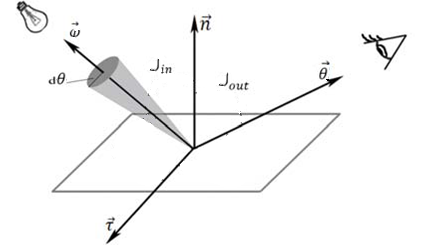
\includegraphics[width=0.499\linewidth]{rendering-equation.png}
\end{center}

Уравнение $(6)$ является частным случаем более общего уравнения, называемого уравнением рендеринга  \cite{rendering-equ}. Существует несколько подходов к его решению. Рассмотрим их.

  \section*{Численный метод}

Численный метод, использованный в работе, описан в \cite{method}. Это конечно-разностный метод, позволяющий найти решение со вторым порядком точности по пространству и с третьим порядком точности по времени. В расчетной области вводится разнесенная, неравномерная сетка. Метод применим только в том случае, если в области можно ввести ортогональную систему координат в которой область представляет из себя паралеллепипед со стенками, параллельными координатным осям. То есть, если $\Omega$~--- расчетная область, то существуют такие отрезки $l_1, l_2, l_3$, что $\Omega = l_1 \times l_2 \times l_3$. 

\begin{figure}
  \begin{center}
    \begin{picture}(180,180)(-90,-90)
      \thinlines
     \put(-90,10){\vector(0,1){40}}
     \put(-90,10){\vector(1,0){40}}
     \put(-90,10){\vector(-1,-1){20}}
     \put(-97,46){\text{z}}
     \put(-56,3){\text{y}}
     \put(-110,-2){\text{x}}
      \thicklines
     \put(-30,-30){\line(0,1){60}}
     \put(-30,30){\line(1,0){60}}
     \put(30,30){\line(0,-1){60}}
     \put(30,-30){\line(-1,0){60}}
     %
     \put(-30,30){\line(1,1){24}}
     \put(30,30){\line(1,1){24}}
     \put(30,-30){\line(1,1){24}}
     %
     \put(-6,54){\line(1,0){60}}
     \put(54,54){\line(0,-1){60}}
      \thinlines
%     \put(-30,-30){\line(1,1){24}}
%    \put(-6,-6){\line(1,0){60}}
%     \put(-6,-6){\line(0,1){60}}
      \thicklines
     \put(0,0){\circle{6}}
     \put(3,-7){\text{$v_x$}}
     \put(42,12){\circle{6}}
     \put(44,5){\text{$v_y$}}
     \put(12,42){\circle{6}}
     \put(15,35){\text{$v_z$}}
     \put(-30,0){\circle*{4}}
     \put(-27,-7){\text{$\omega_z$}}
     \put(0,30){\circle*{4}}
     \put(3,23){\text{$\omega_y$}}
     \put(0,-30){\circle*{4}}
     \put(3,-37){\text{$\omega_y$}}
     \put(30,0){\circle*{4}}
     \put(33,-7){\text{$\omega_z$}}
     \put(54,24){\circle*{4}}
     \put(57,17){\text{$\omega_z$}}
     \put(42,-18){\circle*{4}}
     \put(45,-25){\text{$\omega_x$}}
     \put(42,42){\circle*{4}}
     \put(43,35){\text{$\omega_x$}}
     \put(24,54){\circle*{4}}
     \put(27,47){\text{$\omega_y$}}
     \put(-18,42){\circle*{4}}
     \put(-15,35){\text{$\omega_x$}}
    \end{picture}
  \end{center}
  \caption{Расположение узлов, к которым относятся компоненты векторов скорости и завихренности, на смещенных сетках. Изображена одная ячейка сетки. Давление p определяется в центре ячейки.}
  \label{picStag}
\end{figure}


Для того, что бы ввести неравномерную сетку, используется непрерывная монотонная функция преобразования $ x = x(\xi) $  , отображающая отрезок [0,1] в отрезок [0,1]. 
\begin{gather}
  x(\xi): [0,1] \longrightarrow [0,1]
\end{gather}
Такая функция переведет одномерную равномерную стетку, введеную на отрезке [0,1] в неравномерную. Введем равномерную сетку из $N_x$ ячеек 
\begin{gather}
 \Xi = \{\xi_i = ih, i = \overline{0..N_x}\}, \qquad h = 1 / N_x 
\end{gather}
Под разностной схемой, построенной на разнесенных сетках\footnote{так же разнесенные сетк называют перемежающиеся сетки, или смещенные сетки, Angl.: staggered mash.}, понимают такую, в которой разные неизвестные величины определины в разных узлах. В нашем случае одни неизвестные относятся к узлам сетки, то есть определены на множестве $\Xi$, а другие оносятся к центрам ячеек, и определены, соответственно, на множестве $\Xi_f$
\begin{gather}
 \Xi_f = \{ \xi_i = i*h - h/2, i = \overline{1..N_x} \}, \qquad h = 1/N_x
\end{gather}
Неравномерные сетки $X$ и $X_f$ есть отображение сеток $x(\xi)$ на $\Xi$ под действием преобразования $x(\xi)$
\begin{gather}
 X = x(\Xi) = \{x_i = x(\xi_i), \xi_i \in \Xi\} \\
 X_f = x(\Xi_f) = \{ x_i = x(\xi_i), \xi_i \in \Xi_f \}
\end{gather}

Если переменная определина в центрах ячеек, ее индекс соотвтствует номеру ячейки и меняется от 1 до $N_x$, а если переменная определена в узлах сетки, ее индекс соответствует номеру узла и меняется от 0 до $N_x$.

Далее используется обозначение $f_i = f(x_i) = f(x(\xi_i))$~--- значение неизвестного f в i-ой точке сетки. Если сказанно, что переменная относится к центру ячейки, значит она определена на сетке $\Xi_f$.  

Для произвольной функции f(x) справедливо утверждение:
$$
  \frac{\partial f}{\partial x} = \frac{\partial f}{\partial \xi} \frac{\partial \xi}{\partial x}
$$
Значение производной функии $x(\xi)$ может быть вычисленно точно,так как явный вид вункции известен.
В соответствии с данным утверждением построен разностный оператор дифференцирования $\delta_x$, аппроксимирующий производную со вторым порядко точности
\begin{gather}
 \delta_x f_i = \frac{\partial x(\xi_i)}{\partial \xi} \frac{f(x(\xi_i + h/2)) - f(x(\xi_i - h/2))}{h}  = \frac{\partial f(x_i)}{\partial x} + O(h^2)
\end{gather}

В частном случае, если предположить, что переменная $f$ определена в узлах сетки $ f_i \in F = f(X)$, тогда $\delta_x f$ относится к центрам ячеек и определяется выражением
$$
  (\delta_x f)_i = (f_i - f_{i-1}) \Delta_i, \text{ где } \Delta_i =  \frac{1}{h}\frac{\partial x(h*i - h/2)}{\partial \xi}
$$

Если, наоборот, $f$ определена в центрах ячеек $ f_i \in F = f(X_f)$, тогда $\delta_x f$
относится к узлам сетки и определяется выражением
$$
  (\delta_x f)_i = (f_{i+1} - f_i) \Delta_i, \text{ где } \Delta_i  = \frac{1}{h}\frac{\partial x(h*i)}{\partial \xi}
$$

Также, вводится вырадение для осреднения по пространству произвольной функции f(x) со вторым порядком точности. Оператор осреднения обозначается горизонтальной чертой над функцией. 
$$
  \overline{f}^x_i = \frac{f(x(\xi_i - h/2)) + f(x(\xi_i + h/2))}{2} = f_i + O(h^2)
$$

В нашем случае, если $f$ определена в узлах сетки $f_i \in F = f(X)$, тогда $\overline{f}^x_i$ относится к центрам ячеек и определеляется выражением
$$
  \overline{f}^x_i = \frac{f_{i-1} + f_{i}}{2}
$$

Если $f$ определена в центрах ячеек $f_i \in F = f(X_f)$, тогда $\overline{f}^x_i$ относится к узлам сетки и определяется выражением
$$
  \overline{f}^x_i = \frac{f_i + f_{i+1}}{2}
$$


Далее описанно ведение сетки в трехмерной области. 
По аналогии с парой $\{X,X_f\}$, введены пары сеток $\{Y,Y_f\}$ и $\{Z,Z_f\}$. В нашем случае необходимо вычислить три компоненты вектора скорости, три компоненты вектора завихренности и двление. Давление относится к центрам ячеек, что значит, что оно определено на множестве точек $X_f \times Y_f \times Z_f$.
$$
  P = \{p_{ijk} = p(x_i,y_j,z_k), \text{ при } x_i \in X_f, y_i \in Y_f, z_i \in Z_f\}
$$
Компоненты вектора скорости относятся к центрам граней ячеек, вектор нормали которых сонаправлен с определяемым вектором.
\begin{gather*}
  V_x = \{ v^x_{ijk} = v_x(x_i,y_j,z_k), \text{ при } x_i \in X, y_i \in Y_f, z_i \in Z_f \} \\
  V_y = \{ v^y_{ijk} = v_y(x_i,y_j,z_k), \text{ при } x_i \in X_f, y_i \in Y, z_i \in Z_f \} \\
  V_z = \{ v^z_{ijk} = v_z(x_i,y_j,z_k), \text{ при } x_i \in X, y_i \in Y_f, z_i \in Z \}
\end{gather*}
Компоненты вектора завихренности определяются в центрах ребер ячейки, соноправленных с определяемым вектором. 
\begin{gather*}
  \Omega_x = \{ \omega^x_{ijk} = \omega_x(x_i,y_j,z_k), \text{ при } x_i \in X_f, y_i \in Y, z_i \in Z \} \\
  \Omega_y = \{ \omega^y_{ijk} = \omega_y(x_i,y_j,z_k), \text{ при } x_i \in X, y_i \in Y_f, z_i \in Z \} \\
  \Omega_z = \{ \omega^z_{ijk} = \omega_z(x_i,y_j,z_k), \text{ при } x_i \in X, y_i \in Y, z_i \in Z_f \}
\end{gather*}
Иллюстрация на Рис \ref{picStag}.

Этого достаточно для того, что бы записать разностную аппроксимацию исходной систм уравнений
\begin{gather}
  \delta_x v_x + \delta_y v_y + \delta_z v_z = 0 
  \\
  \omega_x = \delta_y v_z - \delta_z v_y 
  \\
  \omega_y = \delta_z v_x - \delta_x v_z 
  \\
  \omega_z = \delta_x v_y - \delta_y v_x 
  \\
  \frac{\partial v_x}{\partial t} = \frac{1}{y'z'}\left(\overline{\overline{y'v_y}^x z' \omega_z}^y - \overline{\overline{z'v_z}^x y' \omega_y}^z \right) - \delta_x p - \nu (\delta_y \omega_z - \delta_z \omega_y)
  \\
  \frac{\partial v_y}{\partial t} = \frac{1}{x'z'}\left(\overline{\overline{z'v_z}^y x' \omega_x}^z - \overline{\overline{x'v_x}^y z' \omega_z}^x \right) - \delta_y p - \nu (\delta_z \omega_x - \delta_x \omega_z) 
  \\
  \frac{\partial v_z}{\partial t} = \frac{1}{x'y'}\left(\overline{\overline{x'v_x}^z y' \omega_y}^x - \overline{\overline{y'v_y}^z x' \omega_x}^y \right) - \delta_z p - \nu (\delta_x \omega_y - \delta_y \omega_x)
\end{gather}

  \section*{Реализация}

1. ------------Трассировка лучей --------------

Для определения видимости полигона $ \alpha $ из точки $ L $, рассматривается отрезок $ LP $, где $ P $ -- центр полигона. Находятся все пересечения отрезка с полигонами модели (разумеется, многоугольник $ \alpha $ не подлежит рассмотрению). Если таких граней не нашлось, то грань $ \alpha $ считается видимой из точки $ L $, иначе -- невидимой. 

Задача определения пересечения отрезка и многоугольника разбивается на следующие этапы.

1. Определить точку пересечения $ M $ плоскости многоугольника и прямой, содержащей отрезок.

2. Находится ли точка пересечения $ M $ внутри многоугольника.

3. Находится ли точка пересечения $ M $ внутри отрезка.

Несмотря на то, что для достаточно детализированной модели с количеством полигонов в несколько тысяч, данный процесс достаточно трудоемок, в работе программе исходной статьи никакие способы оптимизации не использовались. Способов оптимизации действительно много и сравнение самых популярных можно прочитать в [*].


  \newpage
\section*{Результаты} 

Результатом работы стало программное обеспечение, написанное на языке программирования C, работающее на операционных системах Linux и Windows. Основные возможности программы:

1. Загружать модель из файла (Wavefront OBJ geometry format, .obj) и отображать ее в трехмерном пространстве с использованием технологии OpenGL.

2. Возможность ставить источник излучения в любую точку пространства.

3. Проводить расчеты первичных и вторично-освещенных граней как на GPU (с использованием технологии CUDA), так и на CPU.

4. Сохранять проведенные расчеты в файл (.obj). Дополнительная информация хранится в комментариях особого вида, что, фактически, не повреждает сам файл.

5. Проводить расчет сферы освещения.

6. Возможность делать проекции сферы освещения с сохранением в файл картинки (Bitmap picture, .bmp).

\subsection*{Диффузное и зеркальное}

Как мы уже упомянули, в программе есть возможность задавать функцию ДФО вручную. Рассмотрим работу программы на простом примере: один треугольный полигон (красный) и один точечный источник излучения (желтая сфера). 

Скриншот программы для диффузного рассеивания по Ламберту:

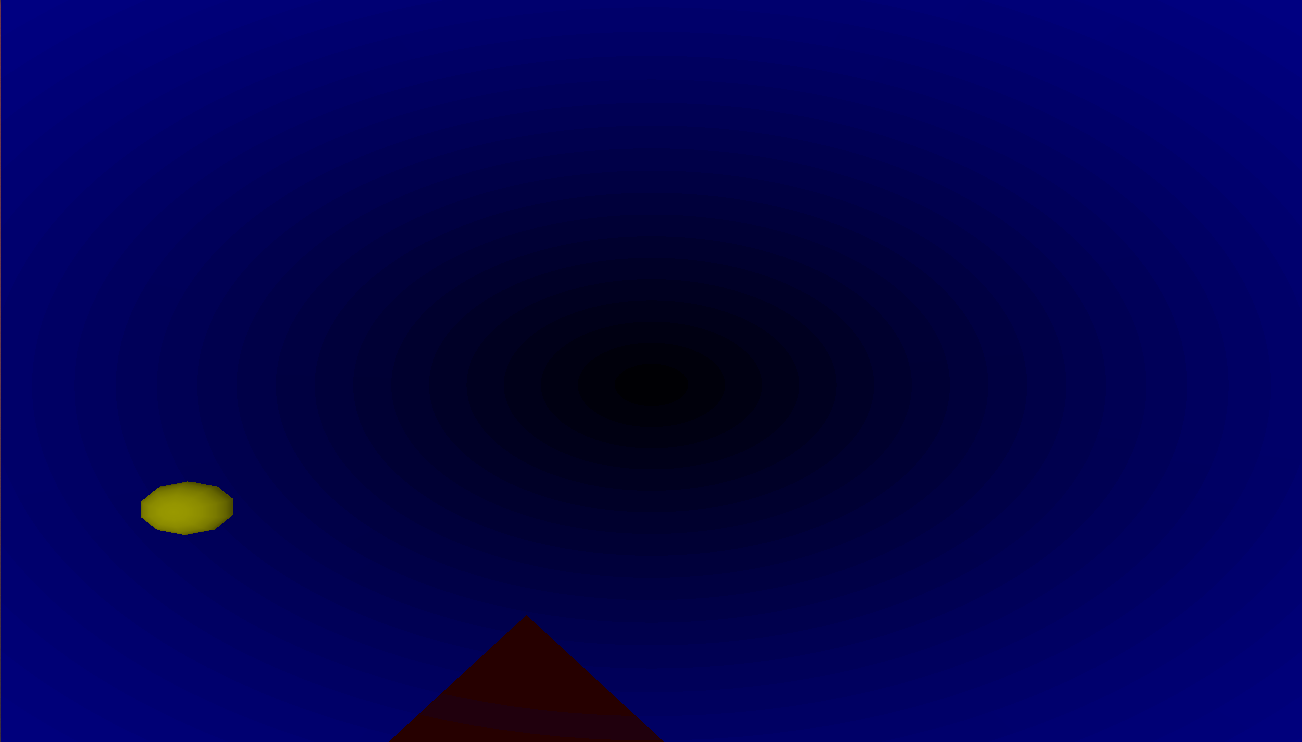
\includegraphics[width=1\linewidth]{lambert-screen.png}

Скриншот программы для зеркального отражения:

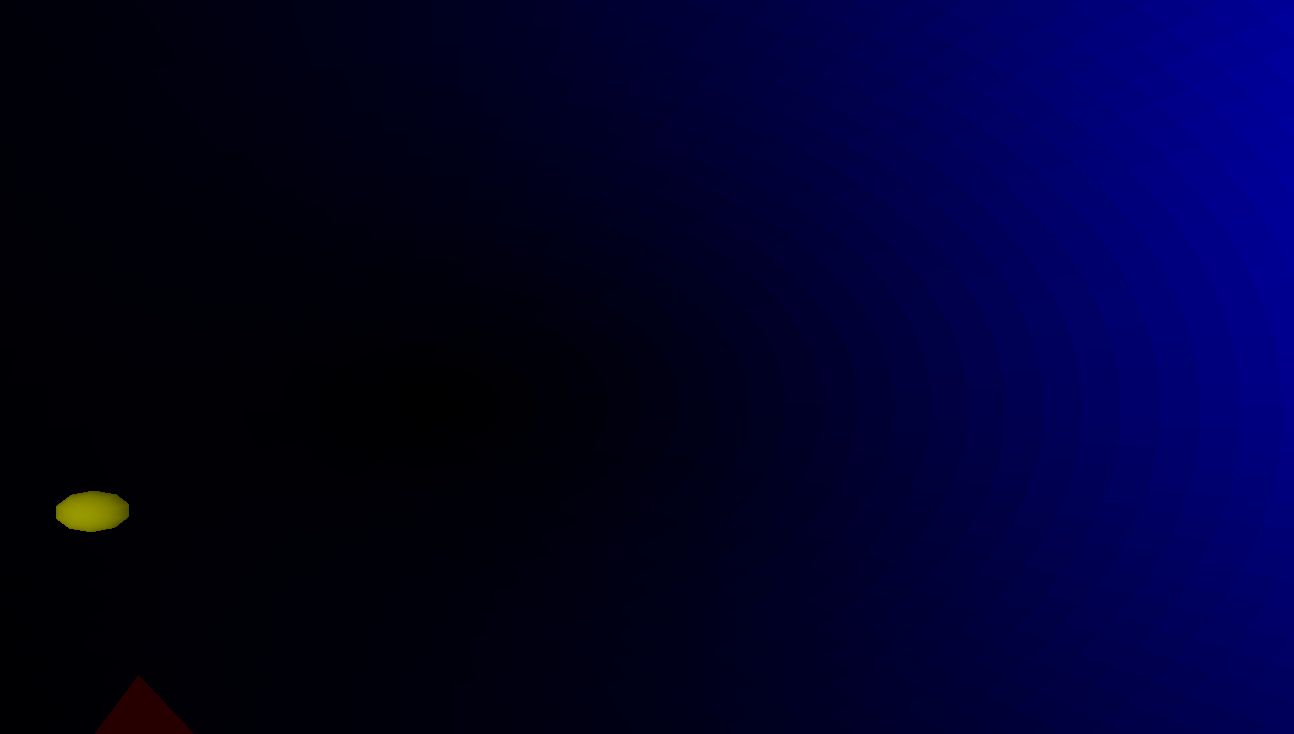
\includegraphics[width=1\linewidth]{zerkalo-screen.png}

Проекции сферы излучения (слева -- диффузное, справа -- зеркальное):

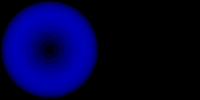
\includegraphics[width=0.499\linewidth]{lambert-map.png}
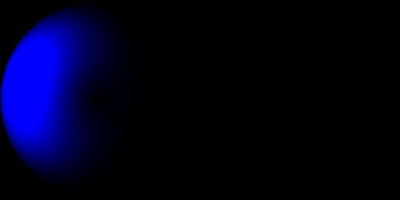
\includegraphics[width=0.499\linewidth]{zerkalo-map.png}

Таким образом, у нас есть возможность достаточно гибко моделировать различные материалы. 

\subsection*{Первичные и вторичные}

Рассмотрим одно положение объектов и сравним разницу между картинами в первом случае создаваемой только первично-освещенными областями и во втором -- совокупностью первичных и вторичных групп полигонов. 

Первично-освещенные области слева, вторичные -- справа:

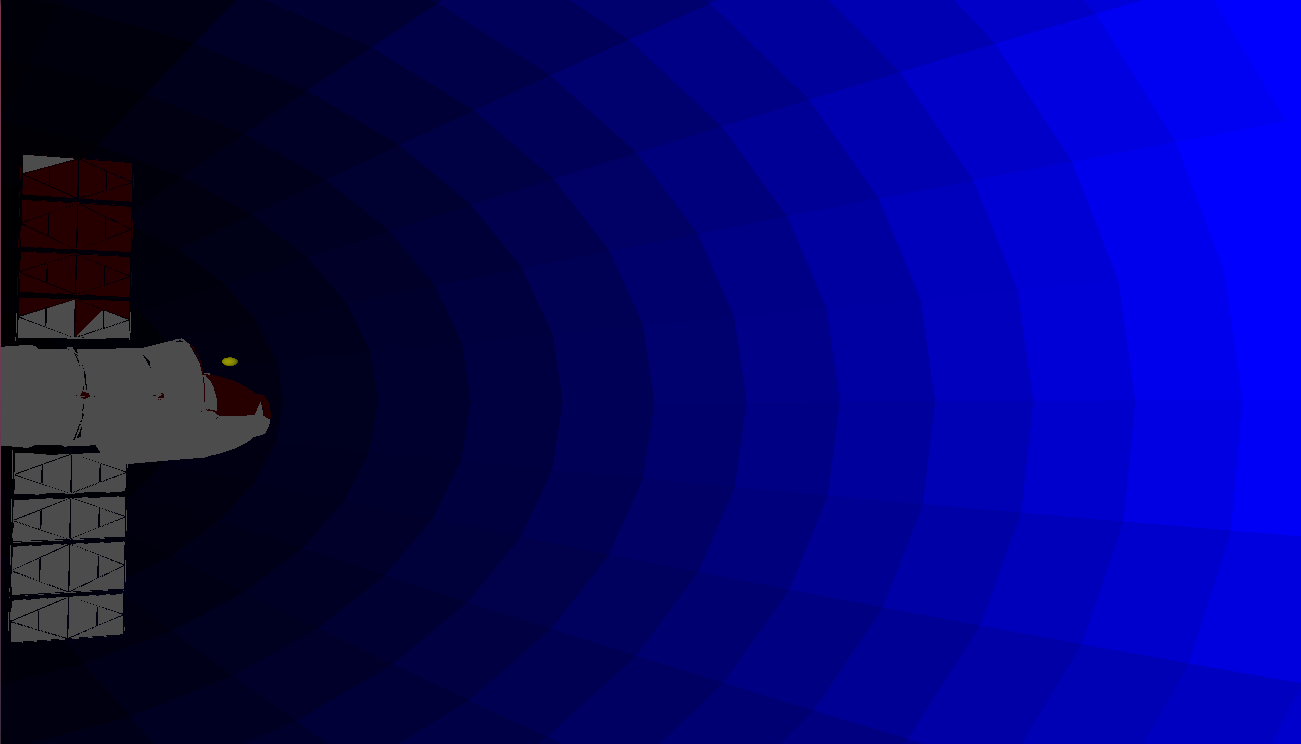
\includegraphics[width=0.499\linewidth]{first-screen-1.png}
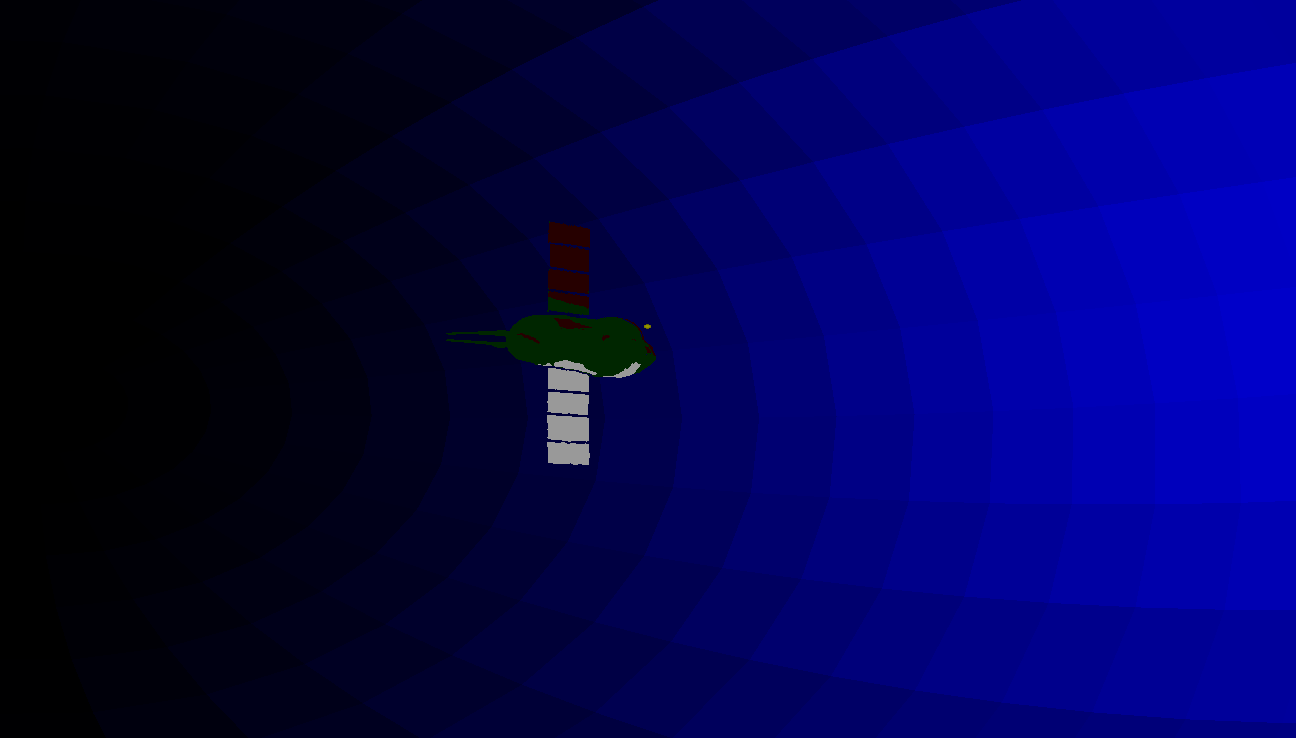
\includegraphics[width=0.499\linewidth]{second-screen-1.png}

Областью $A$ обозначено отражение от верхней антенной части корабля. Область $B$ -- пространство, излучение на карте проекций которого изменилось. 

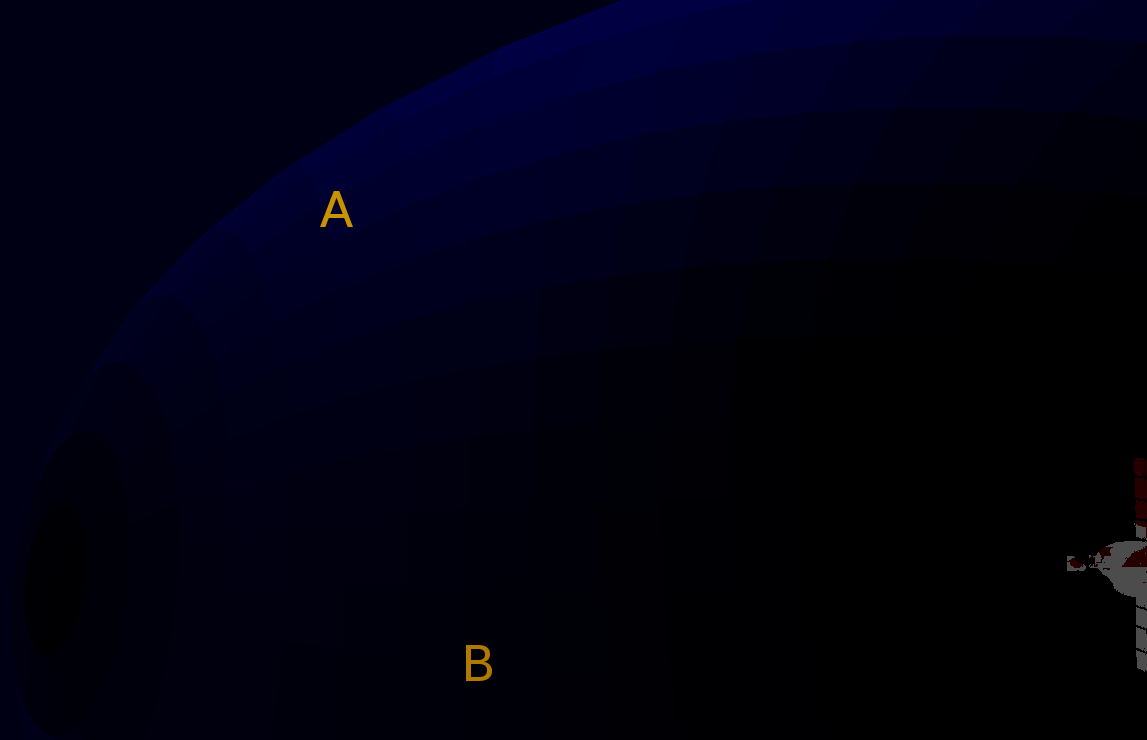
\includegraphics[width=0.51\linewidth]{first-screen-2.png}
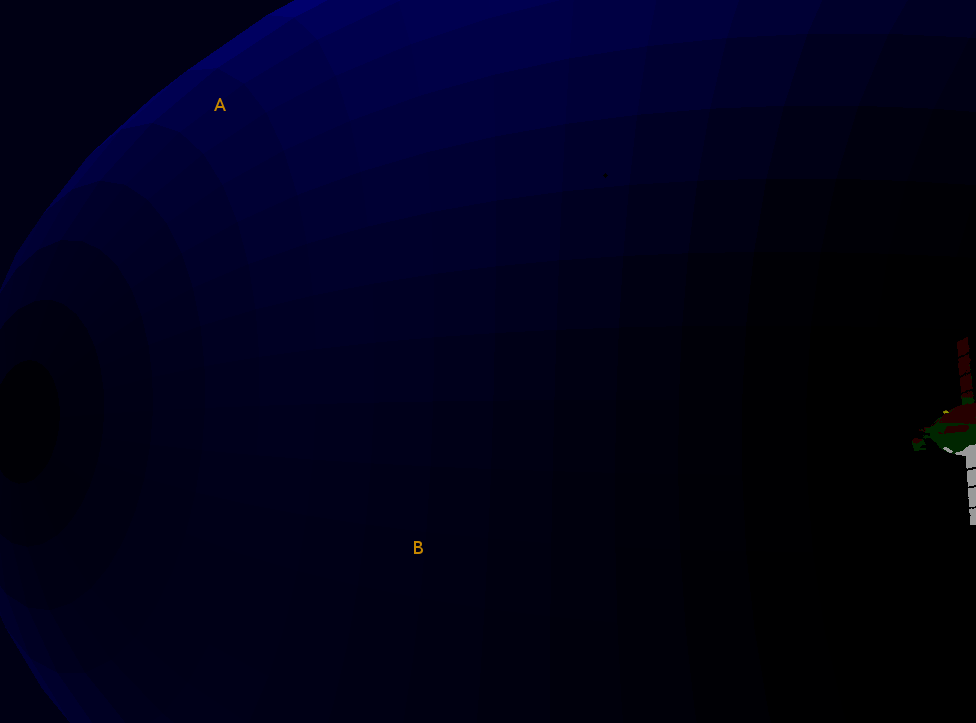
\includegraphics[width=0.445\linewidth]{second-screen-2.png}

Проекции сферы излучения (слева -- только первичные, справа первичные и вторичные области):

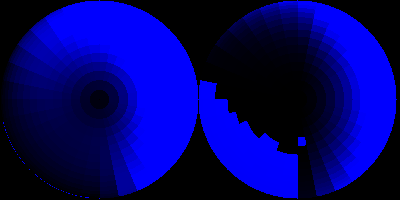
\includegraphics[width=0.499\linewidth]{first-map.png}
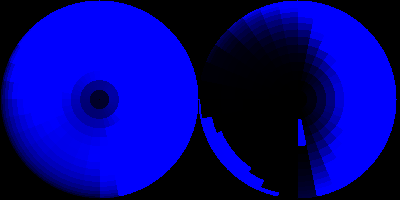
\includegraphics[width=0.499\linewidth]{second-map.png}

По картам заметно, левая нижняя область сферы (область $B$) стала светлее. Таким образом, в этой области существенный вклад вносит вторичное отражение. 

Таким образом, можно анализировать проекции сферы и выявлять области, в которых

1. излучение изменяется под влиянием вторичных зон (либо присутствует только переотраженный сигнал, либо присутствуют оба сигнала, но значения второго оказываются существенными),

2. излучение не подвергается изменениям (значение вторичного сигнала не существенно).

\subsection*{Сравнение производительности}

Проведем сравнение производительностей по моделированию поставленных нами задач. Помимо параллельной версии программы, запускаемой на графическом ускорителе, была написана последовательная версия программы, запускаемая на центральном процессоре.  

Характеристики центрального процессора (CPU): модель Intel Core 2 Duo T6600, тактовая частота 2200 MHz. 

Несмотря на то, что процессор многоядерный, программа была написана последовательно, то есть во время исполнении занято было только одно ядро.

Характеристики графического ускорителя (GPU): чипсет Nvidia GeForse GT 240M, объем 1024 mb.

Сравнение проводилось на трех сложных одинаковых полигональных моделях слонов с разной степенью детализации. Задача на GPU запускалась на сетке 65535 x 512 нитей.

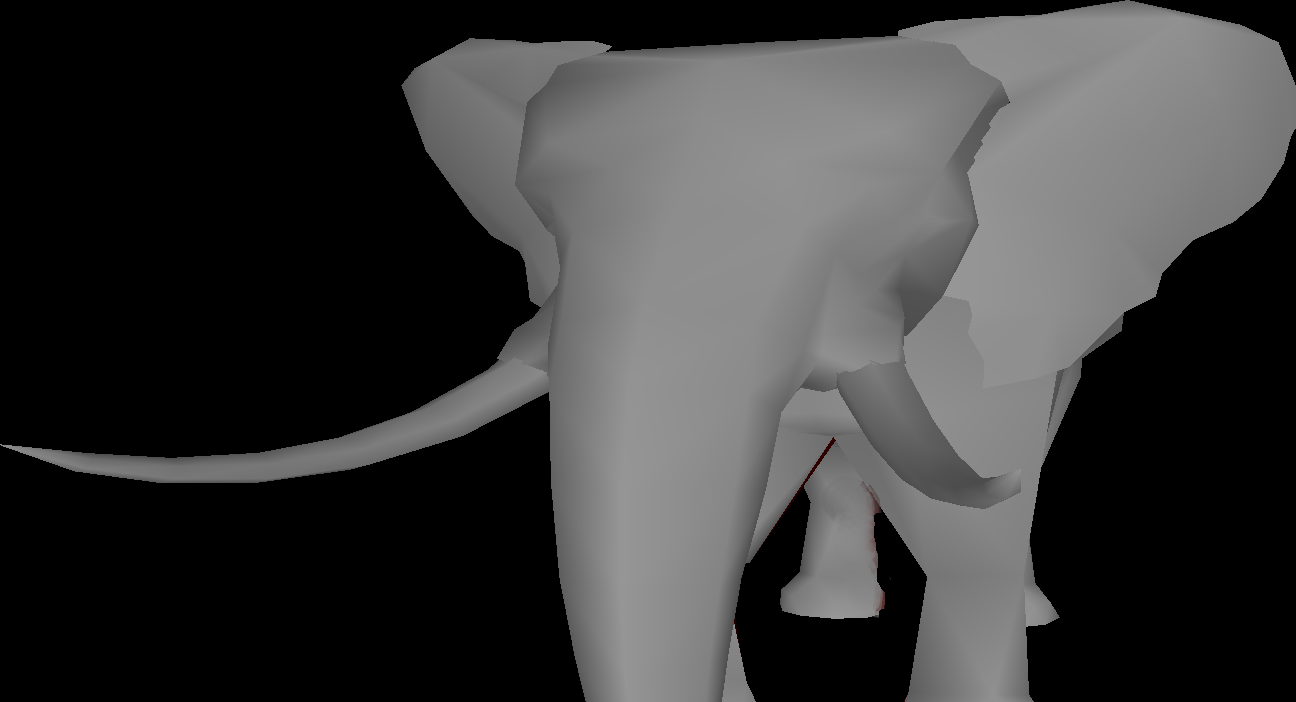
\includegraphics[width=0.28\linewidth]{elephav.png}
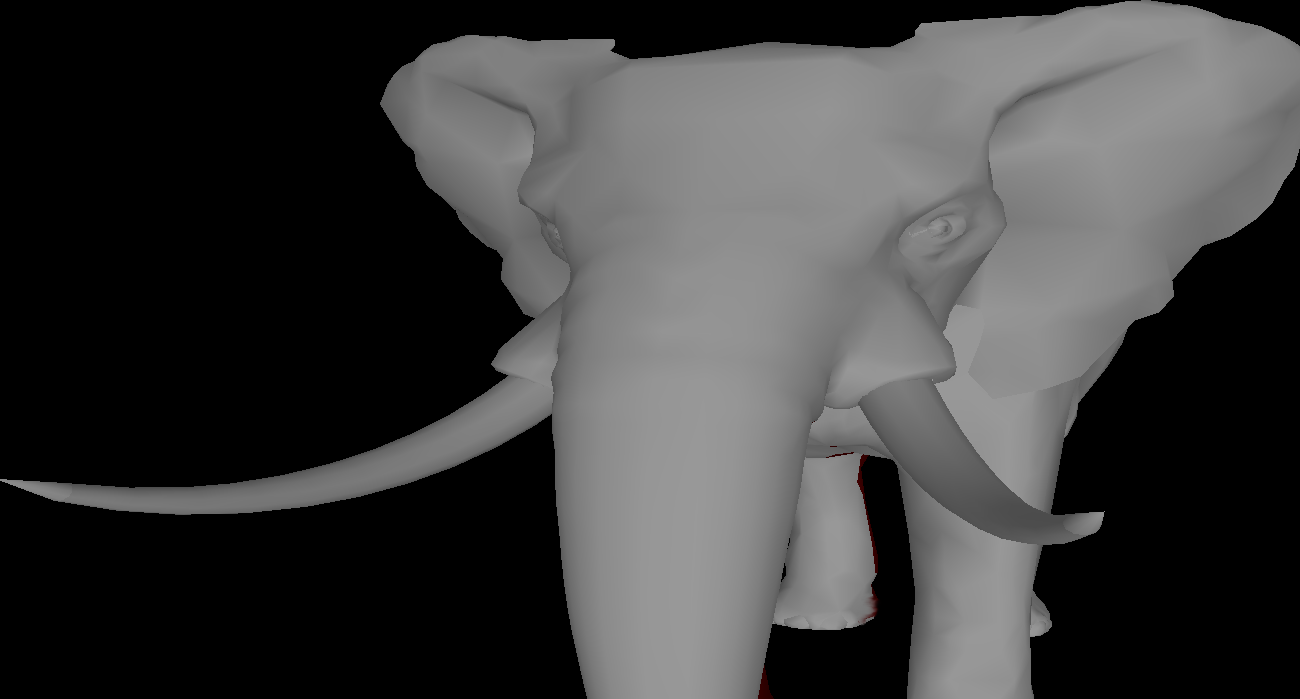
\includegraphics[width=0.28\linewidth]{elephal.png}
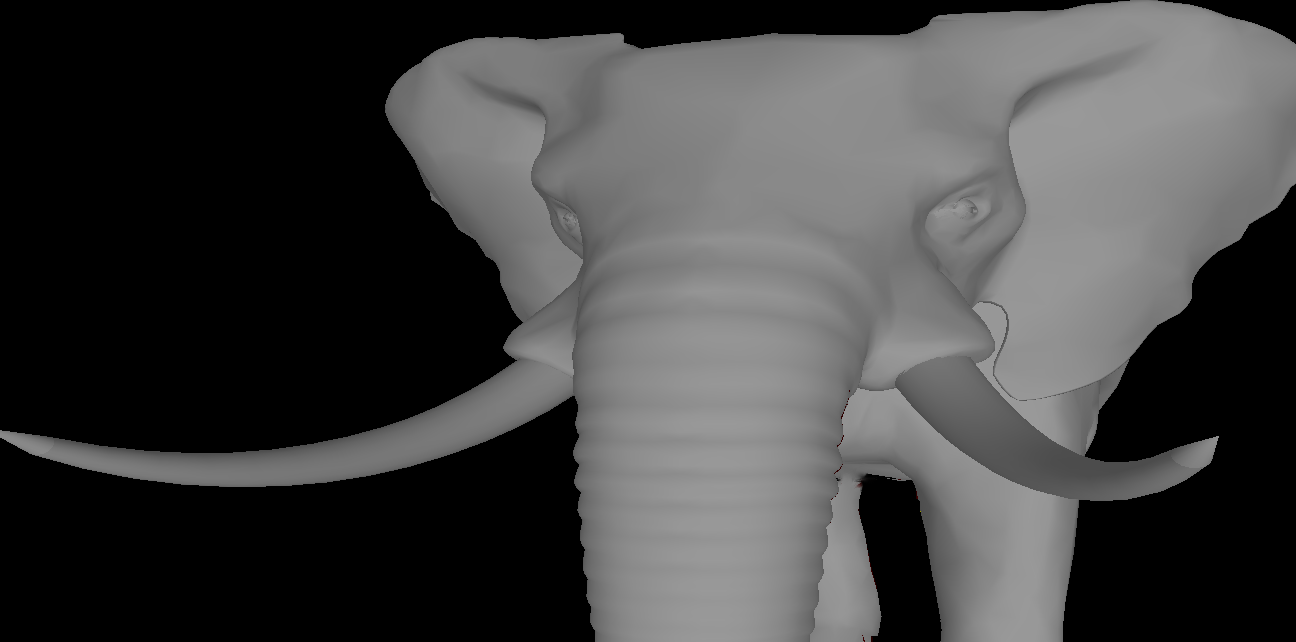
\includegraphics[width=0.305\linewidth]{elepham.png}

\begin{center}
Расчет первичных зон отражения
\begin{tabular}{cccc}
\textbf{время в мс}		& \textbf{слон 1148 гр} 			& \textbf{слон 10152 гр}		& \textbf{слон 39292 гр} 		\\
CPU 							& 172					 				& 16115								& 587850			 						\\
GPU 							& 105									& 	320								& 1292									\\
ускорение 					& 1.63								& 50.36								& 454.99 									\\
\end{tabular}
\end{center}

Таким образом, видно, что чем и крупнее задача, тем сильнее получаем ускорение. 




  \newpage
\begin{thebibliography}{99}

  \bibitem{sazonov}
  \textit{С.Б.\,Медведев, В.В.\,Сазонов, Х.У.\,Сайгираев}, Моделирование зон неустойчивой работы радиотехнической измерительной системы с активным ответом во время сближения и стыковки космических кораблей с Международной Космической Станцией
  // Математическое моделирование, 24(2):151–160, 2012.
  [\href{http://istina.imec.msu.ru/publications/article/533721/}{html}]

  \bibitem{soyz}
  Легедарный корабль <<Союз>>
  // Новости Космонавтики, апрель 2002


  \bibitem{boreskov1}
  \textit{А.В.\,Боресков, А.А.\,Харламов}, Основы работы с технологией CUDA
  // ДМК Пресс, 2010

  \bibitem{berezin}
  \textit{C.Б.\,Березин, В.М.\,Пасконов, Н.А.\,Сахарных}, Моделирование трехмерных течений методом расщепления с использованием параллельной архитектуры ГПУ
 // Вычислительные методы и программирование, 13: 75-81, 2012.
  [\href{http://num-meth.srcc.msu.ru/zhurnal/tom_2012/pdf/v13r210.pdf}{pdf}]

  \bibitem{cynami}
  \textit{М.А.\,Курако}, Оптимизация производительности вычислений для моделирования цунами на параллельных архитекутурах
  // Молодёжь и наука: Сборник материалов VII Всероссийской научно-технической конференции студентов, аспирантов и молодых учёных, посвященной 50-летию первого полета человека в космос
  [\href{http://elib.sfu-kras.ru/bitstream/2311/5869/1/s3_029.pdf}{pdf}]
  
  \bibitem{neuron}
  \textit{В.В.\,Парубец, О.Г.\,Берестнева, Д.В.\,Девятых}, Применение технологии CUDA для ускорения вычислений в нейронных сетях
  // Известия Томского политехнического университета, том 320, выпуск 5 (2012)

  \bibitem{radiolocation}
  \textit{П.В.\,Маковецкий, В.Г.\,Васильев}, Отражение радиолокационных сигналов -- лекции
  // Ленинградский институт авиационного приборостроения, 1975

  \bibitem{gugens}
  Принцип Гюйгенса-Френеля
  // Большая советская энциклопедия (3-е издание)

  \bibitem{ferma}
  \textit{Schuster A.}, An Introduction to the Theory of Optics. 
  //London: Edward Arnold (1904), 340 p.


  \bibitem{frenel}
  \textit{Hecht E.}, Optics. 
  //Addison Wesley, 1987. 457 p.


  \bibitem{lambert}
  \textit{Frank Pedrotti, Leno Pedrotti}, Introduction to Optics. 
  // Prentice Hall, 1993. ISBN 0135015456.  

  \bibitem{rendering-equ}
  \textit{J.\,Kajiya}, The rendering equation
  // ACM SIGGRAPH Computer Graphics, 1986. 20. N 4. P. 143-150

  \bibitem{history}
  \textit{Андрей Лебедев}, История развития алгоритмов глобального освещения
  // Компьютерная графика и мультимедиа, 2011
  [\href{http://cgm.computergraphics.ru/issues/issue19/globalillum}
  {html}]

  \bibitem{ray-tracing}
  \textit{Cook R., Porter T., Carpenter L.}, Distributed ray tracing
  // SIGGRAPH Comput. Graph, 1984. 18. N 3. P. 137-145.

  \bibitem{geometry}
  \textit{Moller T., Trumbore B.}, Fast, Minimum Storage Ray-Triangle Intersection 
  // J. Graphics Tools, 1997, v.2(1), p.21 -- 28.

  \bibitem{brezenhem}
  \textit{Роджерс Д.}, Алгоритмические основы машинной графики
  //Мир, 1989. — С. 512.

  \bibitem{3dda}, Анализ алгоритмов трассировки лучей для реалистичной визуализации трехмерных сцен и способов уменьшения их вычислительной сложности. 

  \textit{И.А. Запорожченко, М.А. Григорьев, С.А. Зори}, 
  //Цифровая обработка сигналов и изображений. – с. 353.
\end{thebibliography}


\end{document}
